\chapter{Las bacterias y la resistencia a los antibióticos}\label{ch:g11:antibiotic-resistance}

En 1941, a un policía que se moría de una septicemia originada en un
arañazo se le administraron las primeras dosis de penicilina que se
usaron nunca en un paciente. Se recuperó en unos días --- y recayó y
murió cuando se agotó el suministro, extraído con enorme esfuerzo de un
moho. En una década la penicilina se fabricaba por toneladas y unas
infecciones que llevaban milenios matando pasaron a curarse en una
semana. En dos décadas, las bacterias a las que la penicilina ya no
tocaba eran corrientes en todos los hospitales. Este capítulo trata del
porqué: de cómo varían las bacterias, de cómo las clasifica un
\omterm{def:g11:antibiotic-resistance:antibiotic}{antibiótico} y de cómo la aritmética de una población de miles de
millones convierte una \omterm{def:g11:mutations:mutation}{mutación} rara en un problema de planta entera.

\begin{omfigure}
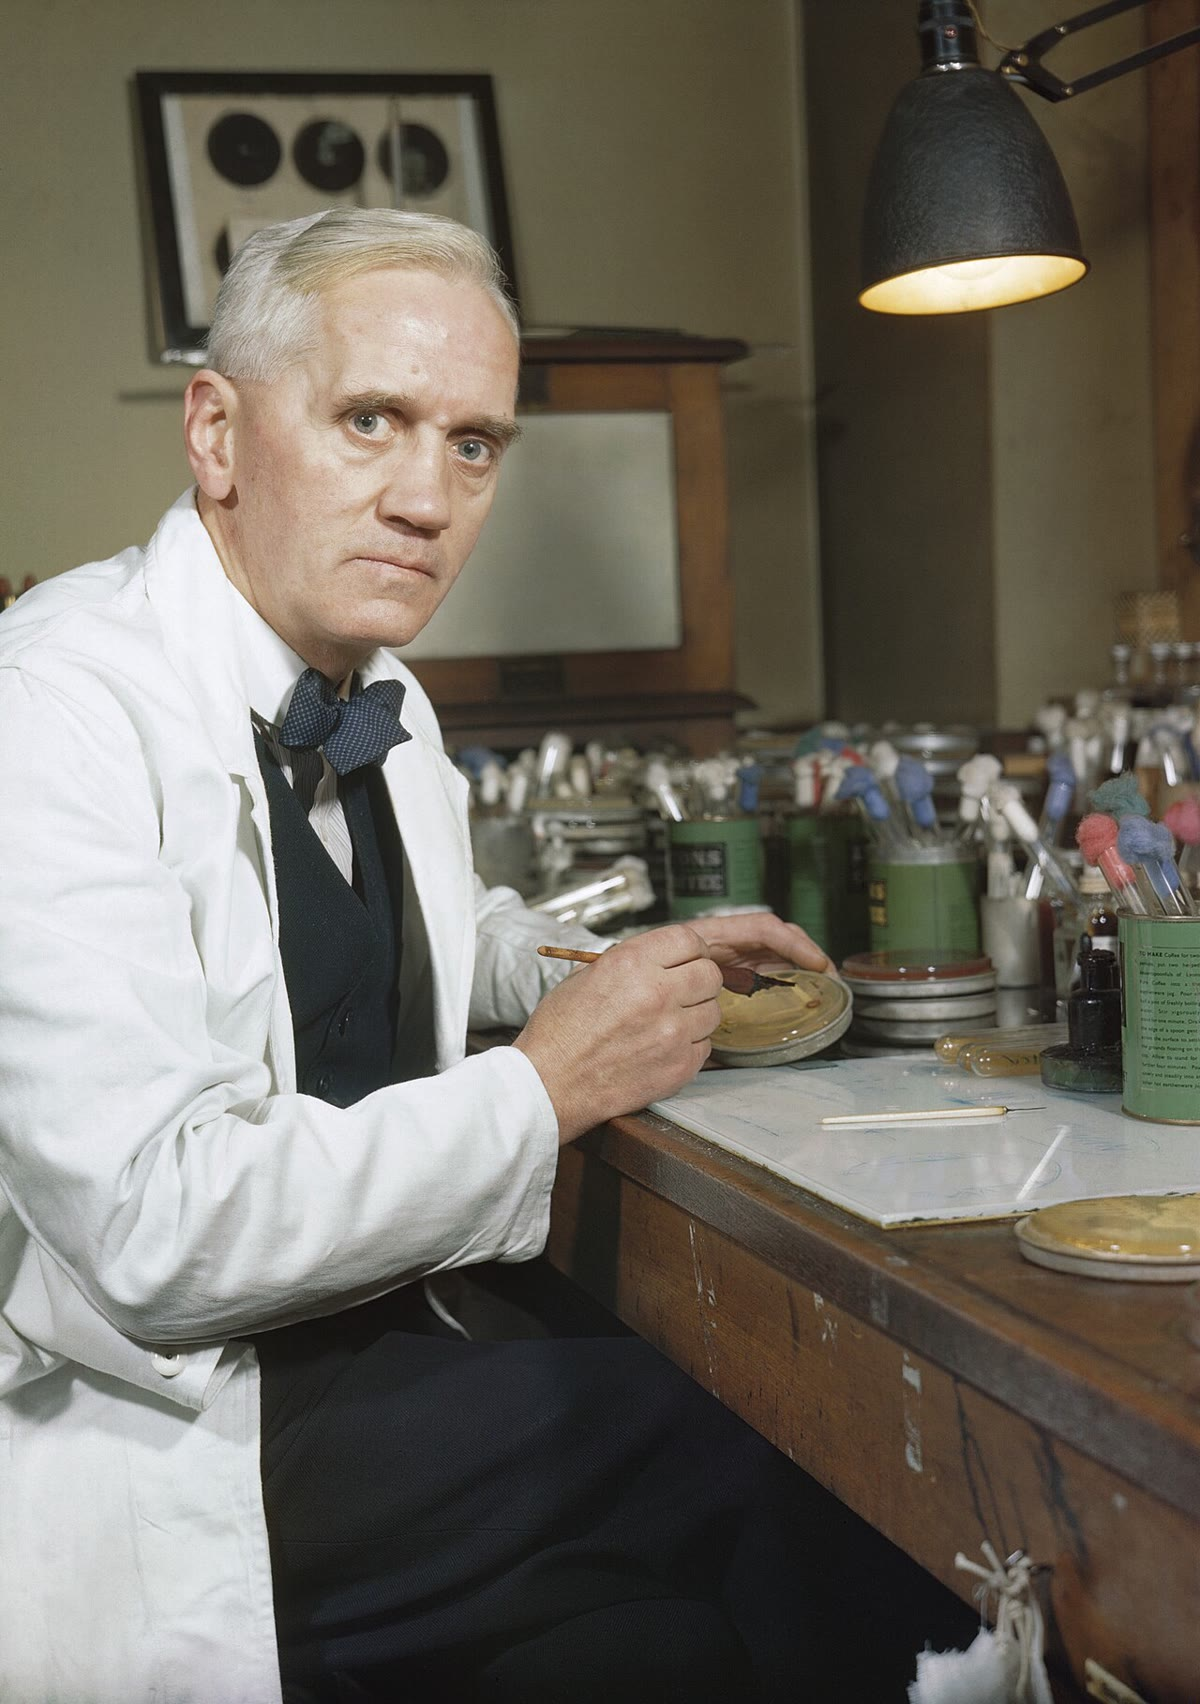
\includegraphics[width=0.4\linewidth]{images/book2/fleming.jpg}

{\small Alexander Fleming en su mesa de trabajo en 1943, con las placas de cultivo en las que, quince años antes, había advertido que un moho aclaraba las bacterias de su alrededor. Fotografía, Imperial War Museums, dominio público.}
\end{omfigure}

\section{Cómo varían las bacterias}

\begin{proposition}[Reproducción y variación bacterianas]\label{prop:g11:antibiotic-resistance:variation}
Una bacteria se reproduce dividiéndose en dos después de copiar su
único \omterm{def:g11:cell-cycle-mitosis:chromosome}{cromosoma}: las hijas son, salvo por los errores de copia,
genéticamente idénticas a la madre --- un \emph{clon}. En un medio
rico, una división cada 20 minutos convierte una \omterm{def:g10:cells-common-unit:cell}{célula} en mil millones
en diez horas. La variación genética del clon procede de dos fuentes:
\begin{itemize}
  \item las \emph{\omterm{def:g11:mutations:mutation}{mutaciones}} (\cref{ch:g11:mutations}), raras por
        división pero frecuentes en una población de miles de millones;
  \item la \emph{transferencia horizontal de genes}\index{transferencia horizontal de genes}:
        \omterm{def:g10:universal-dna:information}{ADN} recibido de otra bacteria, de la misma \omterm{def:g10:biodiversity-scales:species}{especie} o de otra, la
        mayoría de las veces en forma de \emph{plásmido} --- un pequeño
        círculo de \omterm{def:g10:universal-dna:information}{ADN}, separado del \omterm{def:g11:cell-cycle-mitosis:chromosome}{cromosoma}, que lleva unos pocos
        \omterm{def:g10:universal-dna:gene}{genes} y puede pasar de una \omterm{def:g10:cells-common-unit:cell}{célula} a otra por un puente de
        membrana.
\end{itemize}
\end{proposition}
\admitted

\begin{omfigure}
\begin{tikzpicture}[font=\small, >=Stealth]
  % donor
  \draw[thick, fill=omDef!10, rounded corners=12pt] (0,0) rectangle (3,1.5);
  \draw[thick, omDef] (0.4,0.75) .. controls (0.6,1.3) and (2.4,1.3) .. (2.6,0.75) .. controls (2.4,0.2) and (0.6,0.2) .. (0.4,0.75);
  \draw[thick, omThm, fill=omThm!20] (2.2,1.15) circle (0.22);
  \node[anchor=north] at (1.5,-0.1) {donante: tiene el plásmido};
  % recipient
  \draw[thick, fill=omDef!10, rounded corners=12pt] (5,0) rectangle (8,1.5);
  \draw[thick, omDef] (5.4,0.75) .. controls (5.6,1.3) and (7.4,1.3) .. (7.6,0.75) .. controls (7.4,0.2) and (5.6,0.2) .. (5.4,0.75);
  \node[anchor=north] at (6.5,-0.1) {receptora};
  % bridge
  \draw[thick, fill=omProp!30] (3,0.55) rectangle (5,0.95);
  \draw[->, thick, omThm] (3.1,0.75) -- (4.9,0.75);
  \node[anchor=north, font=\scriptsize] at (4,-0.6) {una copia del plásmido cruza el puente};
  % result
  \draw[->, thick] (8.4,0.75) -- (9.2,0.75);
  \draw[thick, fill=omDef!10, rounded corners=12pt] (9.5,0) rectangle (12.5,1.5);
  \draw[thick, omDef] (9.9,0.75) .. controls (10.1,1.3) and (11.9,1.3) .. (12.1,0.75) .. controls (11.9,0.2) and (10.1,0.2) .. (9.9,0.75);
  \draw[thick, omThm, fill=omThm!20] (11.7,1.15) circle (0.22);
  \node[anchor=north, align=center] at (11,-0.1) {la receptora lleva ya\\ los genes del plásmido};
  \node[anchor=west, font=\scriptsize, omDef] at (0.2,1.75) {cromosoma};
  \node[anchor=west, font=\scriptsize, omThm] at (2.5,1.75) {plásmido};
\end{tikzpicture}

{\small Transferencia horizontal. Un plásmido --- un pequeño círculo de
\omterm{def:g10:universal-dna:information}{ADN} que puede llevar un \omterm{def:g10:universal-dna:gene}{gen} de resistencia --- se copia a través de un
puente de una bacteria a otra, que no tiene por qué ser de la misma
\omterm{def:g10:biodiversity-scales:species}{especie}. La receptora, y todos sus descendientes, ganan el \omterm{def:g10:universal-dna:gene}{gen} de una
sola vez.}
\end{omfigure}

\begin{example}[La aritmética de una población]\label{ex:g11:antibiotic-resistance:arithmetic}
Una \omterm{def:g11:mutations:mutation}{mutación} de resistencia surge más o menos una vez cada $10^8$
divisiones. Un matraz con $10^9$ bacterias ha tenido, por tanto, en las
divisiones que lo produjeron, unas diez \omterm{def:g11:mutations:mutation}{mutaciones} así; una herida
infectada o un intestino, con $10^{12}$ bacterias, unas diez mil. Toda
población grande de bacterias contiene, antes de usar ningún
\omterm{def:g11:antibiotic-resistance:antibiotic}{antibiótico}, \omterm{def:g10:cells-common-unit:cell}{células} \omterm{prop:g11:antibiotic-resistance:mechanisms}{resistentes} a él --- las placas de réplica del
\cref{ch:g11:mutations} lo demostraron.
\end{example}

\section{Los antibióticos}

\begin{definition}[Antibiótico]\label{def:g11:antibiotic-resistance:antibiotic}
Un \emph{antibiótico}\index{antibiótico} es una molécula que mata a las
bacterias o detiene su crecimiento, a concentraciones inofensivas para
las \omterm{def:g10:cells-common-unit:cell}{células} del paciente, actuando sobre una estructura o un proceso
que las bacterias tienen y las \omterm{def:g10:cells-common-unit:cell}{células} humanas no: la penicilina y sus
parientes bloquean la construcción de la pared bacteriana; la
estreptomicina y la tetraciclina atascan el \omterm{def:g10:cells-common-unit:organelle}{ribosoma} bacteriano, que es
distinto del nuestro; otros bloquean las \omterm{def:g11:enzymes-and-phenotype:enzyme}{enzimas} bacterianas de la
\omterm{def:g11:dna-replication:replication}{replicación del ADN}. Casi todos se encontraron primero en mohos y en
bacterias del suelo, que los fabrican contra sus competidores. Los
antibióticos no tienen ningún efecto sobre los virus, que no poseen
ninguna de esas dianas.
\end{definition}

\begin{proposition}[Mecanismos de resistencia]\label{prop:g11:antibiotic-resistance:mechanisms}
Una bacteria es \emph{resistente}\index{resistencia a los antibióticos}
a un \omterm{def:g11:antibiotic-resistance:antibiotic}{antibiótico} cuando crece a concentraciones que detienen a sus
parientes sensibles. La resistencia tiene una base genética de unos
pocos tipos: un \omterm{def:g10:universal-dna:gene}{gen} de una \omterm{def:g11:enzymes-and-phenotype:enzyme}{enzima} que destruye el \omterm{def:g11:antibiotic-resistance:antibiotic}{antibiótico} (las
penicilinasas cortan la penicilina en dos); una \omterm{def:g11:mutations:mutation}{mutación} que altera la
diana del \omterm{def:g11:antibiotic-resistance:antibiotic}{antibiótico} de modo que el fármaco ya no se una (una \omterm{def:g11:gene-expression:protein}{proteína}
ribosómica cambiada); una bomba que expulsa el fármaco; una pared que
no lo deja entrar. Cada uno es un \omterm{def:g10:universal-dna:gene}{alelo} o un \omterm{def:g10:universal-dna:gene}{gen}, y cada uno se hereda
--- verticalmente por el clon y, cuando está en un plásmido,
horizontalmente por las vecinas.
\end{proposition}
\admitted

\begin{method}[Leer un antibiograma]\label{met:g11:antibiotic-resistance:antibiogram}
Un \emph{antibiograma} prueba las bacterias de un paciente frente a
varios \omterm{def:g11:antibiotic-resistance:antibiotic}{antibióticos} a la vez.
\begin{enumerate}
  \item Se siembran las bacterias de manera uniforme en una placa; se
        colocan discos de papel empapados cada uno en un \omterm{def:g11:antibiotic-resistance:antibiotic}{antibiótico};
        se incuba una noche.
  \item El \omterm{def:g11:antibiotic-resistance:antibiotic}{antibiótico} difunde desde el disco y su concentración baja
        con la distancia; las bacterias crecen formando un césped
        salvo donde la concentración las detiene: un \emph{halo de
        inhibición} transparente alrededor de cada disco.
  \item Se mide el diámetro de cada halo y se compara con el umbral
        establecido para ese \omterm{def:g11:antibiotic-resistance:antibiotic}{antibiótico}: un diámetro por encima del
        umbral significa sensible, y por debajo, \omterm{prop:g11:antibiotic-resistance:mechanisms}{resistente}.
  \item Los halos mayores entre los resultados sensibles guían la
        prescripción; un disco sin ningún halo es un \omterm{def:g11:antibiotic-resistance:antibiotic}{antibiótico} que la
        cepa ignora.
\end{enumerate}
\end{method}

\begin{omfigure}
\begin{tikzpicture}[font=\small]
  \draw[thick, fill=omProp!12] (0,0) circle (3.7);
  \foreach \a/\r/\l in {90/1.3/A, 162/0.9/B, 234/0.0/C, 306/1.6/D, 18/0.55/E} {
    \begin{scope}[shift={(\a:2.0)}]
      \ifdim \r pt > 0pt \draw[fill=white] (0,0) circle (\r); \fi
      \draw[fill=gray!30] (0,0) circle (0.28);
      \node[font=\scriptsize] at (0,0) {\l};
    \end{scope}
  }
  \node[anchor=west, align=left] at (3.8,1.6) {A: halo \qty{26}{mm}, umbral 17: sensible};
  \node[anchor=west, align=left] at (3.8,0.9) {B: halo \qty{18}{mm}, umbral 20: resistente};
  \node[anchor=west, align=left] at (3.8,0.2) {C: sin halo: resistente};
  \node[anchor=west, align=left] at (3.8,-0.5) {D: halo \qty{32}{mm}, umbral 22: sensible};
  \node[anchor=west, align=left] at (3.8,-1.2) {E: halo \qty{11}{mm}, umbral 15: resistente};
  \node[anchor=north, align=center] at (0,-3.9) {césped de bacterias del paciente;\\ discos claros de agar alrededor de los discos de antibiótico};
\end{tikzpicture}

{\small Un antibiograma leído. Cada disco contiene un \omterm{def:g11:antibiotic-resistance:antibiotic}{antibiótico}; el
halo transparente es donde las bacterias no han podido crecer.
Comparados con el umbral de cada fármaco, los diámetros clasifican la
cepa como sensible a A y a D y \omterm{prop:g11:antibiotic-resistance:mechanisms}{resistente} a B, C y E.}
\end{omfigure}

\begin{omfigure}
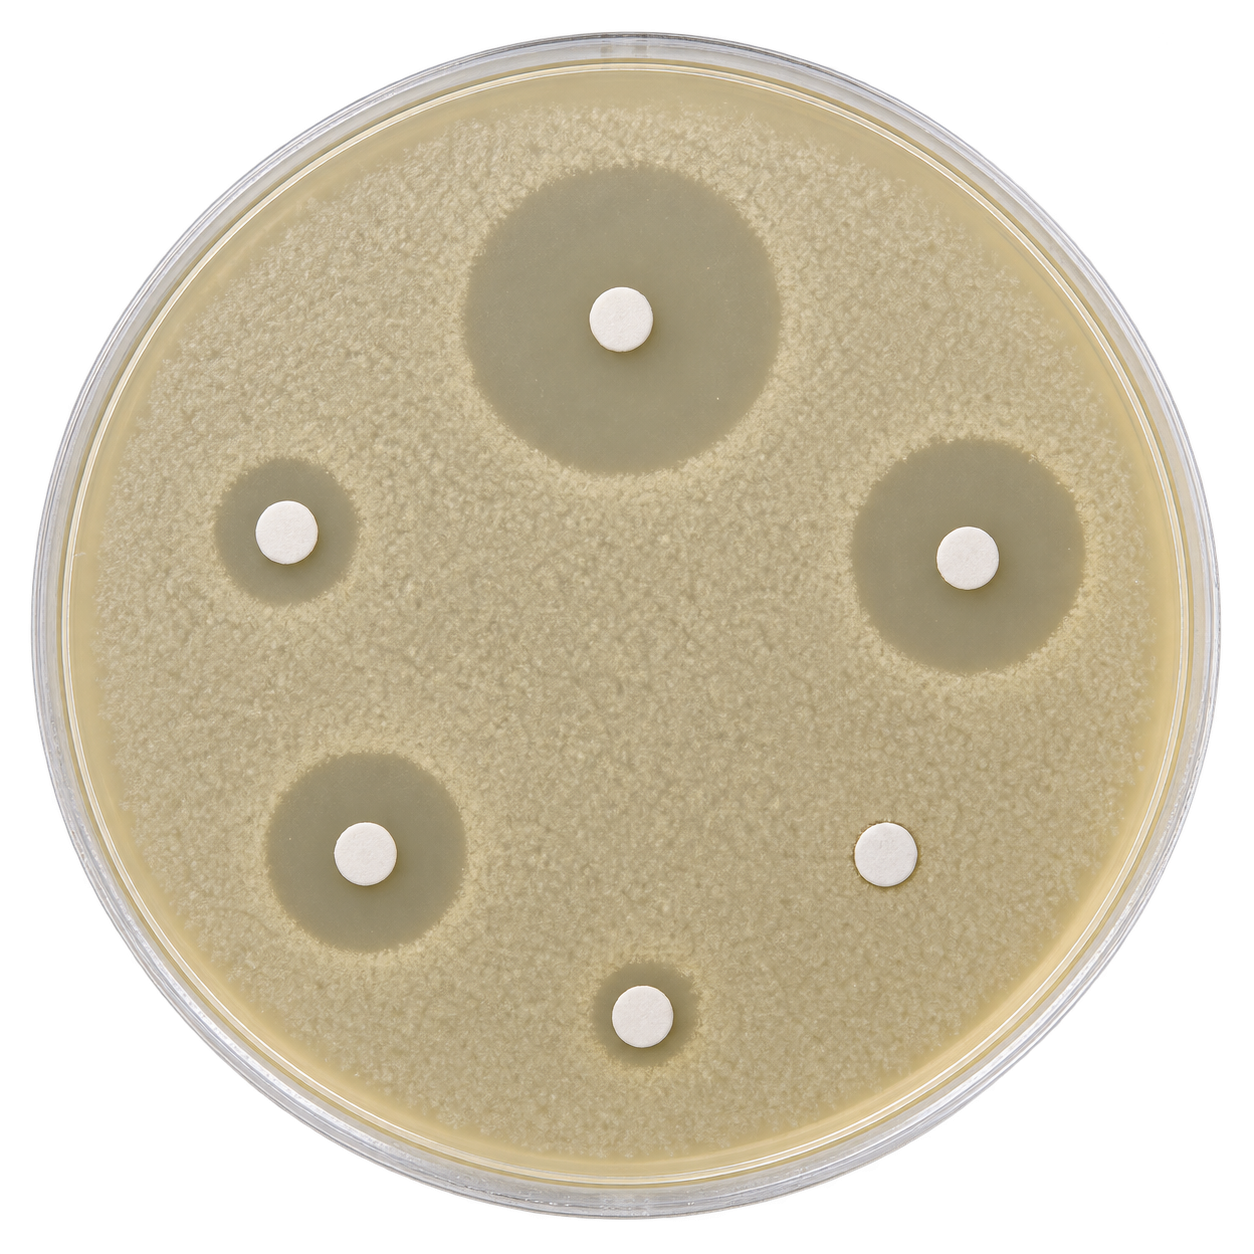
\includegraphics[width=0.44\linewidth]{images/book2/ai/g11-antibiogram-plate.png}

{\small Una placa de antibiograma tras una noche de incubación: un
césped de bacterias y, alrededor de cada disco de \omterm{def:g11:antibiotic-resistance:antibiotic}{antibiótico}, un halo
transparente cuyo tamaño mide la sensibilidad de la cepa. Un disco no
tiene halo.}
\end{omfigure}

\section{Cómo se extiende la resistencia}

\begin{proposition}[La selección por el antibiótico]\label{prop:g11:antibiotic-resistance:selection}
Un \omterm{def:g11:antibiotic-resistance:antibiotic}{antibiótico} no crea bacterias \omterm{prop:g11:antibiotic-resistance:mechanisms}{resistentes}; las
\emph{selecciona}. En una población donde unas pocas \omterm{def:g10:cells-common-unit:cell}{células} llevan un
\omterm{def:g10:universal-dna:gene}{alelo} de resistencia, el fármaco mata o detiene a la mayoría sensible y
deja que las pocas \omterm{prop:g11:antibiotic-resistance:mechanisms}{resistentes} se multipliquen sin competencia: en
unos días la población es \omterm{prop:g11:antibiotic-resistance:mechanisms}{resistente}. Cuanto más se usa un \omterm{def:g11:antibiotic-resistance:antibiotic}{antibiótico}
--- en pacientes, en animales, en el ambiente ---, más a menudo ocurre
esa clasificación, y más \omterm{prop:g11:antibiotic-resistance:mechanisms}{resistentes} se vuelven las bacterias de un
hospital, de una granja o de un país. Una tanda incompleta, que mata a
las \omterm{def:g10:cells-common-unit:cell}{células} más sensibles y perdona a las menos, es la que selecciona
con más eficacia de todas.
\end{proposition}
\begin{proof}[Pruebas experimentales]
Las placas de réplica de Lederberg mostraron que las \omterm{def:g10:cells-common-unit:cell}{células}
\omterm{prop:g11:antibiotic-resistance:mechanisms}{resistentes} ya estaban ahí antes de la exposición. Los cultivos
mantenidos una semana en concentraciones crecientes de un \omterm{def:g11:antibiotic-resistance:antibiotic}{antibiótico}
acaban resistiendo cien veces la dosis inicial, y su resistencia se
hereda y se localiza en \omterm{def:g11:mutations:mutation}{mutaciones} concretas. Los países que más
\omterm{def:g11:antibiotic-resistance:antibiotic}{antibióticos} usan por habitante tienen las proporciones más altas de
cepas \omterm{prop:g11:antibiotic-resistance:mechanisms}{resistentes}; las plantas hospitalarias que reducen su uso ven
bajar la resistencia en unos meses. Una cepa de la bacteria de la piel
\emph{Staphylococcus aureus} \omterm{prop:g11:antibiotic-resistance:mechanisms}{resistente} a la penicilina apareció a los
cuatro años de la introducción del fármaco y hoy representa la mayoría
de las cepas hospitalarias; la cepa \omterm{prop:g11:antibiotic-resistance:mechanisms}{resistente} al fármaco que la
sustituyó llegó dos años después que él.
\end{proof}

\begin{omfigure}
\begin{tikzpicture}
\begin{axis}[
  width=0.88\linewidth, height=5.8cm,
  axis x line=bottom, axis y line=left,
  xmin=0, xmax=6, ymin=0, ymax=110,
  xlabel={días de tratamiento}, ylabel={bacterias (\% del inicio)},
  xlabel style={font=\small, at={(axis description cs:0.5,-0.12)}, anchor=north},
  ylabel style={font=\small},
  tick label style={font=\small}, xtick={0,1,2,3,4,5,6}, ytick={0,25,50,75,100},
  legend style={at={(0.5,-0.3)}, anchor=north, legend columns=3, font=\small, draw=none},
  clip=false,
]
\addplot[thick, omDef] coordinates {(0,100) (0.5,45) (1,15) (1.5,5) (2,1.5) (3,0.2) (4,0.05) (5,0.01) (6,0)};
\addplot[thick, omThm] coordinates {(0,0.001) (1,0.01) (2,0.1) (3,1) (4,8) (5,40) (6,100)};
\addplot[thick, omMeth, dashed] coordinates {(0,100) (0.5,45) (1,15) (1.5,5) (2,1.5) (3,1.2) (4,9) (5,48) (6,100)};
\legend{células sensibles, resistentes (una de cada $10^5$), total si se corta el día 3}
\end{axis}
\end{tikzpicture}

{\small La selección durante una tanda de \omterm{def:g11:antibiotic-resistance:antibiotic}{antibiótico}. Las \omterm{def:g10:cells-common-unit:cell}{células}
sensibles (azul) mueren en unos días; las pocas \omterm{prop:g11:antibiotic-resistance:mechanisms}{resistentes} (rojo) se
multiplican sin oposición y, al final de la semana, forman toda la
población. Si el paciente lo deja el día 3, los supervivientes vuelven
a crecer --- y ahora son casi todos \omterm{prop:g11:antibiotic-resistance:mechanisms}{resistentes}.}
\end{omfigure}

\begin{example}[De una célula a una planta entera]\label{ex:g11:antibiotic-resistance:ward}
Un paciente tratado con penicilina lleva, entre $10^{10}$ bacterias,
un centenar de \omterm{prop:g11:antibiotic-resistance:mechanisms}{resistentes}. En tres días las sensibles han desaparecido
y el clon \omterm{prop:g11:antibiotic-resistance:mechanisms}{resistente} ha ocupado su sitio: $10^{10}$ \omterm{def:g10:cells-common-unit:cell}{células}
\omterm{prop:g11:antibiotic-resistance:mechanisms}{resistentes}. En las manos de una enfermera, en la barandilla de una
cama, en el paciente de al lado, el clon continúa --- y si su \omterm{def:g10:universal-dna:gene}{gen} de
resistencia está en un plásmido, se lo entrega por el camino a otras
\omterm{def:g10:biodiversity-scales:species}{especies}. Nada de esta secuencia exigió que el \omterm{def:g11:antibiotic-resistance:antibiotic}{antibiótico} actuara
sobre el \omterm{def:g10:universal-dna:information}{ADN}; solo retiró la competencia.
\end{example}

\section{Que los antibióticos sigan funcionando}

\begin{proposition}[Consecuencias y respuestas]\label{prop:g11:antibiotic-resistance:consequences}
Las infecciones \omterm{prop:g11:antibiotic-resistance:mechanisms}{resistentes} son más largas, más caras y más a menudo
mortales; algunas cepas resisten ya a todos los fármacos disponibles.
Como la resistencia la impulsa el uso, la respuesta es usar los
\omterm{def:g11:antibiotic-resistance:antibiotic}{antibióticos} menos y mejor: solo para infecciones bacterianas (nunca
para resfriados ni gripes, que son víricos), elegidos tras un
antibiograma cuando sea posible, a dosis completa durante toda la
tanda y con el fármaco de espectro más estrecho que funcione; limitar
su uso en ganadería; prevenir las infecciones (higiene, vacunación)
para que hagan falta menos tandas; y aislar en los hospitales a los
portadores de cepas \omterm{prop:g11:antibiotic-resistance:mechanisms}{resistentes}. Los \omterm{def:g11:antibiotic-resistance:antibiotic}{antibióticos} nuevos ganan tiempo;
la aritmética de la selección garantiza que aparecerá resistencia a
cada uno de ellos.
\end{proposition}
\admitted

\begin{remark}[Evolución en una semana]\label{rem:g11:antibiotic-resistance:evolution}
La \omterm{def:g11:mutations:mutation}{mutación} que aporta variación al azar, el ambiente que la clasifica
y los descendientes de los supervivientes que heredan la diferencia:
las bacterias de este capítulo recorren, en una semana, el proceso que
el último año describirá a lo largo de millones de años para las
ballenas y los robles. La \omterm{prop:g11:antibiotic-resistance:mechanisms}{resistencia a los antibióticos} es evolución
por selección natural observada en tiempo real, con el ser humano como
agente que selecciona --- y la demostración más clara de que el proceso
no es una teoría sobre el pasado, sino un hecho de cualquier población
que varíe y se reproduzca.
\end{remark}

\section{Ejercicios}

\begin{exercise}[$\star$]\label{exo:g11:antibiotic-resistance:1}
Nombra las dos fuentes de variación genética de una población
bacteriana.
\end{exercise}

\begin{exercise}[$\star$]\label{exo:g11:antibiotic-resistance:2}
¿Qué es un \omterm{def:g11:antibiotic-resistance:antibiotic}{antibiótico} y por qué daña a las bacterias y no a las
\omterm{def:g10:cells-common-unit:cell}{células} del paciente? ¿Por qué es inútil contra un resfriado?
\end{exercise}

\begin{exercise}[$\star$]\label{exo:g11:antibiotic-resistance:3}
Da tres mecanismos por los que una bacteria puede resistir a un
\omterm{def:g11:antibiotic-resistance:antibiotic}{antibiótico}.
\end{exercise}

\begin{exercise}[$\star$]\label{exo:g11:antibiotic-resistance:4}
En la figura del antibiograma, un disco nuevo F da un halo de
\qty{20}{mm} con un umbral de \qty{18}{mm}. ¿Sensible o \omterm{prop:g11:antibiotic-resistance:mechanisms}{resistente}?
¿Qué \omterm{def:g11:antibiotic-resistance:antibiotic}{antibiótico} recetarías de la A a la F?
\end{exercise}

\begin{exercise}[$\star$]\label{exo:g11:antibiotic-resistance:5}
¿Causa un \omterm{def:g11:antibiotic-resistance:antibiotic}{antibiótico} las \omterm{def:g11:mutations:mutation}{mutaciones} de resistencia? Justifícalo con el
experimento del \cref{ch:g11:mutations}.
\end{exercise}

\begin{exercise}[$\star\star$]\label{exo:g11:antibiotic-resistance:6}
Partiendo de una bacteria que se divide cada 20 minutos, ¿cuántas hay
al cabo de 10 horas? Si la resistencia surge una vez cada $10^8$
divisiones, ¿cuántas \omterm{def:g10:cells-common-unit:cell}{células} \omterm{prop:g11:antibiotic-resistance:mechanisms}{resistentes} contiene probablemente el
cultivo?
\end{exercise}

\begin{exercise}[$\star\star$]\label{exo:g11:antibiotic-resistance:7}
En la figura de la selección, ¿en qué día pasan a ser mayoría del total
las \omterm{def:g10:cells-common-unit:cell}{células} \omterm{prop:g11:antibiotic-resistance:mechanisms}{resistentes}? ¿Cuál es la población total el día 6 en el caso
de la línea discontinua, y de qué está formada?
\end{exercise}

\begin{exercise}[$\star\star$]\label{exo:g11:antibiotic-resistance:8}
Explica por qué un \omterm{def:g10:universal-dna:gene}{gen} de resistencia situado en un plásmido se
extiende más deprisa que uno situado en el \omterm{def:g11:cell-cycle-mitosis:chromosome}{cromosoma}.
\end{exercise}

\begin{exercise}[$\star\star$]\label{exo:g11:antibiotic-resistance:9}
Un paciente se encuentra mejor al tercer día de una tanda de siete y la
deja. Explica, con la figura, qué ocurre en los días siguientes y por
qué la recaída es más difícil de tratar.
\end{exercise}

\begin{exercise}[$\star\star$]\label{exo:g11:antibiotic-resistance:10}
¿Por qué la proporción de cepas \omterm{prop:g11:antibiotic-resistance:mechanisms}{resistentes} es mayor en los hospitales
que en la población general?
\end{exercise}

\begin{exercise}[$\star\star$]\label{exo:g11:antibiotic-resistance:11}
Explica por qué una \omterm{def:g11:mutations:mutation}{mutación} que altera una \omterm{def:g11:gene-expression:protein}{proteína} ribosómica puede
hacer \omterm{prop:g11:antibiotic-resistance:mechanisms}{resistente} a la estreptomicina a una bacteria, y por qué esa
bacteria suele crecer algo más despacio que sus parientes sensibles.
\end{exercise}

\begin{exercise}[$\star\star\star$]\label{exo:g11:antibiotic-resistance:12}
Se administran juntos dos \omterm{def:g11:antibiotic-resistance:antibiotic}{antibióticos} con dianas distintas. Estima la
probabilidad de que una \omterm{def:g10:cells-common-unit:cell}{célula} sea \omterm{prop:g11:antibiotic-resistance:mechanisms}{resistente} a los dos por \omterm{def:g11:mutations:mutation}{mutaciones}
independientes (una de cada $10^8$ para cada una) y explica por qué se
usa la terapia combinada contra infecciones lentas y largas como la
tuberculosis.
\end{exercise}

\begin{exercise}[$\star\star\star$]\label{exo:g11:antibiotic-resistance:13}
Una granja añade dosis bajas de un \omterm{def:g11:antibiotic-resistance:antibiotic}{antibiótico} al pienso para acelerar
el crecimiento. Predice las consecuencias para las bacterias de los
animales, para los trabajadores de la granja y para la medicina humana,
usando la selección y la transferencia horizontal.
\end{exercise}

\begin{exercise}[$\star\star\star$]\label{exo:g11:antibiotic-resistance:14}
Una planta hospitalaria reduce a la mitad sus prescripciones de
\omterm{def:g11:antibiotic-resistance:antibiotic}{antibióticos}; en un año baja la proporción de cepas \omterm{prop:g11:antibiotic-resistance:mechanisms}{resistentes}.
Explica por qué la resistencia puede retroceder, usando el coste que la
resistencia tiene para la bacteria y la competencia.
\end{exercise}

\begin{exercise}[$\star\star\star$]\label{exo:g11:antibiotic-resistance:15}
``Las bacterias se vuelven \omterm{prop:g11:antibiotic-resistance:mechanisms}{resistentes} porque se acostumbran al
\omterm{def:g11:antibiotic-resistance:antibiotic}{antibiótico}.'' Reescribe correctamente esta frase, en un párrafo corto,
usando la \omterm{def:g11:mutations:mutation}{mutación}, la selección y la herencia.
\end{exercise}

\section{Problema: La planta}

\begin{problem}[{Problema de fin de semana --- un brote en una planta
hospitalaria seguido desde una única célula mutante: la aritmética de
una colonia, un antibiograma leído, una tanda interrumpida y la
política que detiene la propagación}]
\label{pb:g11:antibiotic-resistance:1}
La herida de un paciente está infectada por $10^{10}$ bacterias de una
sola \omterm{def:g10:biodiversity-scales:species}{especie}. Las bacterias se dividen cada 30 minutos; una \omterm{def:g11:mutations:mutation}{mutación}
que da resistencia al \omterm{def:g11:antibiotic-resistance:antibiotic}{antibiótico} amoxicilina ocurre una vez cada
$10^8$ divisiones. El \omterm{def:g11:antibiotic-resistance:antibiotic}{antibiótico} mata al 90\% de las \omterm{def:g10:cells-common-unit:cell}{células} sensibles
cada 6 horas y no afecta a las \omterm{prop:g11:antibiotic-resistance:mechanisms}{resistentes}, que siguen dividiéndose.

\medskip
\noindent\textbf{Parte I --- Antes del tratamiento.}
\begin{enumerate}
  \item ¿Cuántas divisiones produjeron las $10^{10}$ bacterias a partir
        de la primera \omterm{def:g10:cells-common-unit:cell}{célula}? (Cuenta el número de \omterm{def:g10:cells-common-unit:cell}{células}.)
  \item Estima el número de \omterm{def:g10:cells-common-unit:cell}{células} \omterm{prop:g11:antibiotic-resistance:mechanisms}{resistentes} presentes antes de
        administrar ningún \omterm{def:g11:antibiotic-resistance:antibiotic}{antibiótico}.
  \item Explica por qué, aun así, la infección del paciente se describe
        como ``sensible'' en el antibiograma.
  \item El antibiograma muestra halos de \qty{24}{mm} para la
        amoxicilina (umbral 17), de \qty{12}{mm} para la eritromicina
        (umbral 20) y ninguno para la penicilina. Interpreta los tres
        resultados.
  \item El médico receta amoxicilina durante 7 días. ¿Por qué no
        penicilina, y por qué no el fármaco de mayor halo si alguno
        hubiera sido mayor?
\end{enumerate}

\medskip
\noindent\textbf{Parte II --- Durante el tratamiento.}
\begin{enumerate}[resume]
  \item ¿Cuántas \omterm{def:g10:cells-common-unit:cell}{células} sensibles quedan al cabo de 1 día? ¿Y al cabo
        de 3?
  \item Partiendo de tu respuesta a la pregunta 2, ¿cuántas \omterm{def:g10:cells-common-unit:cell}{células}
        \omterm{prop:g11:antibiotic-resistance:mechanisms}{resistentes} hay al cabo de 1 día si se duplican cada 30 minutos
        sin límite? (Usa $2^{48} \approx \num{2.8e14}$.) ¿Por qué es
        irreal esa cifra y qué la limita?
  \item Supón que el clon \omterm{prop:g11:antibiotic-resistance:mechanisms}{resistente} está limitado al espacio que dejan
        libre las \omterm{def:g10:cells-common-unit:cell}{células} sensibles, de modo que no puede pasar de
        $10^{10}$. ¿Cuándo llena aproximadamente ese espacio?
  \item Esboza, o describe, las curvas de \omterm{def:g10:cells-common-unit:cell}{células} sensibles,
        \omterm{prop:g11:antibiotic-resistance:mechanisms}{resistentes} y totales a lo largo de los 7 días.
  \item En realidad, el sistema inmunitario del paciente elimina en
        unos días los últimos millones de \omterm{def:g10:cells-common-unit:cell}{células} de cualquier clase.
        Explica por qué el desenlace depende de que el clon \omterm{prop:g11:antibiotic-resistance:mechanisms}{resistente}
        crezca más deprisa de lo que el sistema inmunitario lo elimina.
\end{enumerate}

\medskip
\noindent\textbf{Parte III --- La tanda interrumpida.}
\begin{enumerate}[resume]
  \item El paciente lo deja al cabo de 2 días, porque se encuentra
        bien. ¿Cuántas \omterm{def:g10:cells-common-unit:cell}{células} sensibles quedan, y qué fracción de la
        población superviviente es \omterm{prop:g11:antibiotic-resistance:mechanisms}{resistente}?
  \item Las bacterias vuelven a crecer hasta $10^{10}$ en los días
        siguientes. ¿Qué proporción es ahora \omterm{prop:g11:antibiotic-resistance:mechanisms}{resistente}, si las \omterm{def:g10:cells-common-unit:cell}{células}
        \omterm{prop:g11:antibiotic-resistance:mechanisms}{resistentes} y las sensibles crecen al mismo ritmo?
  \item El paciente recae y se le vuelve a dar amoxicilina. Predice el
        resultado.
  \item Un antibiograma de la recaída no muestra ningún halo para la
        amoxicilina. Explica el cambio respecto del primer
        antibiograma.
  \item El \omterm{def:g10:universal-dna:gene}{gen} de resistencia está en un plásmido. ¿Qué riesgo añadido
        supone eso para la planta?
\end{enumerate}

\medskip
\noindent\textbf{Parte IV --- La política de la planta.}
La planta trata a 400 pacientes al año con amoxicilina; el 30\% de las
infecciones aisladas en ella son ya \omterm{prop:g11:antibiotic-resistance:mechanisms}{resistentes}, frente al 5\% en la
ciudad.
\begin{enumerate}[resume]
  \item Explica la diferencia entre la planta y la ciudad en términos
        de presión de selección.
  \item La planta decide: antibiograma antes de toda prescripción,
        tandas completas, higiene de manos y aislamiento de los
        portadores de cepas \omterm{prop:g11:antibiotic-resistance:mechanisms}{resistentes}. Di sobre qué mecanismo de este
        capítulo actúa cada medida.
  \item Al cabo de dos años, la resistencia en la planta es del 12\%.
        Explica por qué bajó y por qué no volvió al 5\%.
  \item ¿Por qué un \omterm{def:g11:antibiotic-resistance:antibiotic}{antibiótico} nuevo, introducido en la planta, no
        resolvería el problema más que unos pocos años?
  \item Enuncia el resultado: el número de \omterm{def:g10:cells-common-unit:cell}{células} \omterm{prop:g11:antibiotic-resistance:mechanisms}{resistentes} que
        tenía la herida antes de todo fármaco, el día en que lo
        heredaron y el único hábito del paciente que convirtió una
        infección curable en un brote.
\end{enumerate}
\end{problem}
